\chapter{What additional calibration can buy}
\label{ci:entry}

Detecting a departure from equilibrium and measuring total dissipation are
different tasks. The previous virtual laboratories made detection more
reliable. The next question is which further observations make a physical
requirement stronger, and which missing information remains inaccessible even
after the statistics improve.

This development follows that question through a complete chain. A calibrated
detector variance shrinks the family of reversible explanations. A nonlinear
information projection measures separation from that smaller family, with
independently checked upper and lower bounds on the numerical relaxation.
A separately calibrated transition-activity cap strengthens the conversion
from record information to required entropy production. Sequential learning
and dependent-record methods address the cost of collecting the evidence.
Explicit countermodels identify the conclusions these improvements cannot buy.

The record-information argument also transfers to a stated class of stationary
overdamped diffusions. Its path-probability identity follows from established
stochastic calculus, while the reversible comparison retains the same positive
spectral structure. This extends the applicable dynamics beyond finite jump
networks. The additional finite-jump activity bound has a narrower domain and
is not transferred to a diffusion by renaming its parameters.

\section{Three boundaries that should not be conflated}
The first boundary is observational. Two physical mechanisms may produce
identical accessible records. More samples cannot distinguish those exact
alternatives. The second is statistical: different record laws may be too
close at the available precision or acquisition budget. The third is a
physical inverse problem: a sharp information certificate need not equal the
smallest entropy production compatible with every dynamical constraint.
Improving an optimization algorithm addresses none of these boundaries by
itself.

The new calibration results supply a concrete example of the first boundary.
Finite positive-lag binary pairs can agree exactly while the detector's
conditional second moment differs. Genuine additional calibration can
therefore change which explanation is admissible. A noisy analog record can
sometimes provide a useful upper variance bound without being a perfect
measurement of the hidden state.

The upper-dissipation obstruction is stronger. A connected four-state cycle
can expose every jump time while concealing the directional marks carrying
its entropy. Even complete microscopic records of bounded duration cannot
uniformly furnish finite upper entropy bounds over models with arbitrarily
rare reverse transitions. This is not a universal cap on scientific data.
It is a target-specific limitation with explicit access and calibration
repairs.

\section{From proofs to acquisition choices}
Calibrated comparison methods, longer observation windows, more readouts and
additional control information have different physical costs. The experiments
therefore report time and readout counts separately. A hypothetical conversion
between these resources is labeled as such; unmeasured hardware expenditure
is not assigned zero cost. Failed regimes and stronger comparators remain in
the evaluation.

The last step moves beyond simulated data. Publicly released optical-tweezer
trajectories are loaded with verified provenance and analyzed using the same
access questions. Their descriptive correlations and detector comparisons
are genuine reanalyses of existing measurements. The available metadata do
not establish all premises of a thermodynamic confidence certificate, so the
analysis records that limitation instead of manufacturing a dissipation claim.
The result is a precise account of what the next laboratory calibration must
supply.

The broad contribution remains operational: connect accessible evidence to
what every admissible physical explanation requires, expose the assumptions
that make the connection valid, and construct the next measurement when those
assumptions are insufficient. Established probability, spectral and
thermodynamic ingredients are credited throughout. Historical priority of the
specific synthesis and independent physical confirmation remain open.

\section{Choosing the next observation}
The most useful next step depends on the obstruction already established.
The following sequence makes that diagnosis explicit.
\begin{enumerate}
\item Specify the target. Detecting departure from detailed balance, lower
bounding entropy production, and upper bounding total entropy are distinct
inverse problems. A method adequate for the first can fail at the other two.
\item Validate the observation contract. Establish how the detector responds,
whether readings disturb the state, how time is recorded, and which source
of independence or dependence control justifies the statistical calculation.
If those conditions are missing, collect calibration evidence before
interpreting a positive contrast physically.
\item Test whether additional access removes an exact ambiguity. Same-state
twins, bounded analog values, directional transition marks and controlled
interventions reveal different information. More repetitions of an exactly
uninformative record cannot substitute for the missing observation.
\item Use all the retained evidence under a valid confidence construction.
A predeclared joint contrast can combine calibration and dynamics. A
nonlinear projection can extract a stronger bound from a covered region.
Predictable sequential tests can stop when sufficient evidence accumulates.
Their conclusions remain limited by the physical comparison theorem.
\item Compare acquisition designs using the resources the apparatus actually
consumes. Report evolution time and readout count before converting to
energy. A microscopic activity cap can sharpen a bound on dissipation; it
does not measure detector power, laser expenditure or initialization work.
\end{enumerate}

This is also a way to decide when a branch is finished. An exact compatible
countermodel settles an impossibility claim for its stated record class.
A covered positive certificate settles a conditional lower-bound claim.
Neither establishes the complete hidden dynamics. A physical application is
complete only when the apparatus supports the premises and the result answers
the stated target at the required precision.

\begin{figure}[p]
\centering
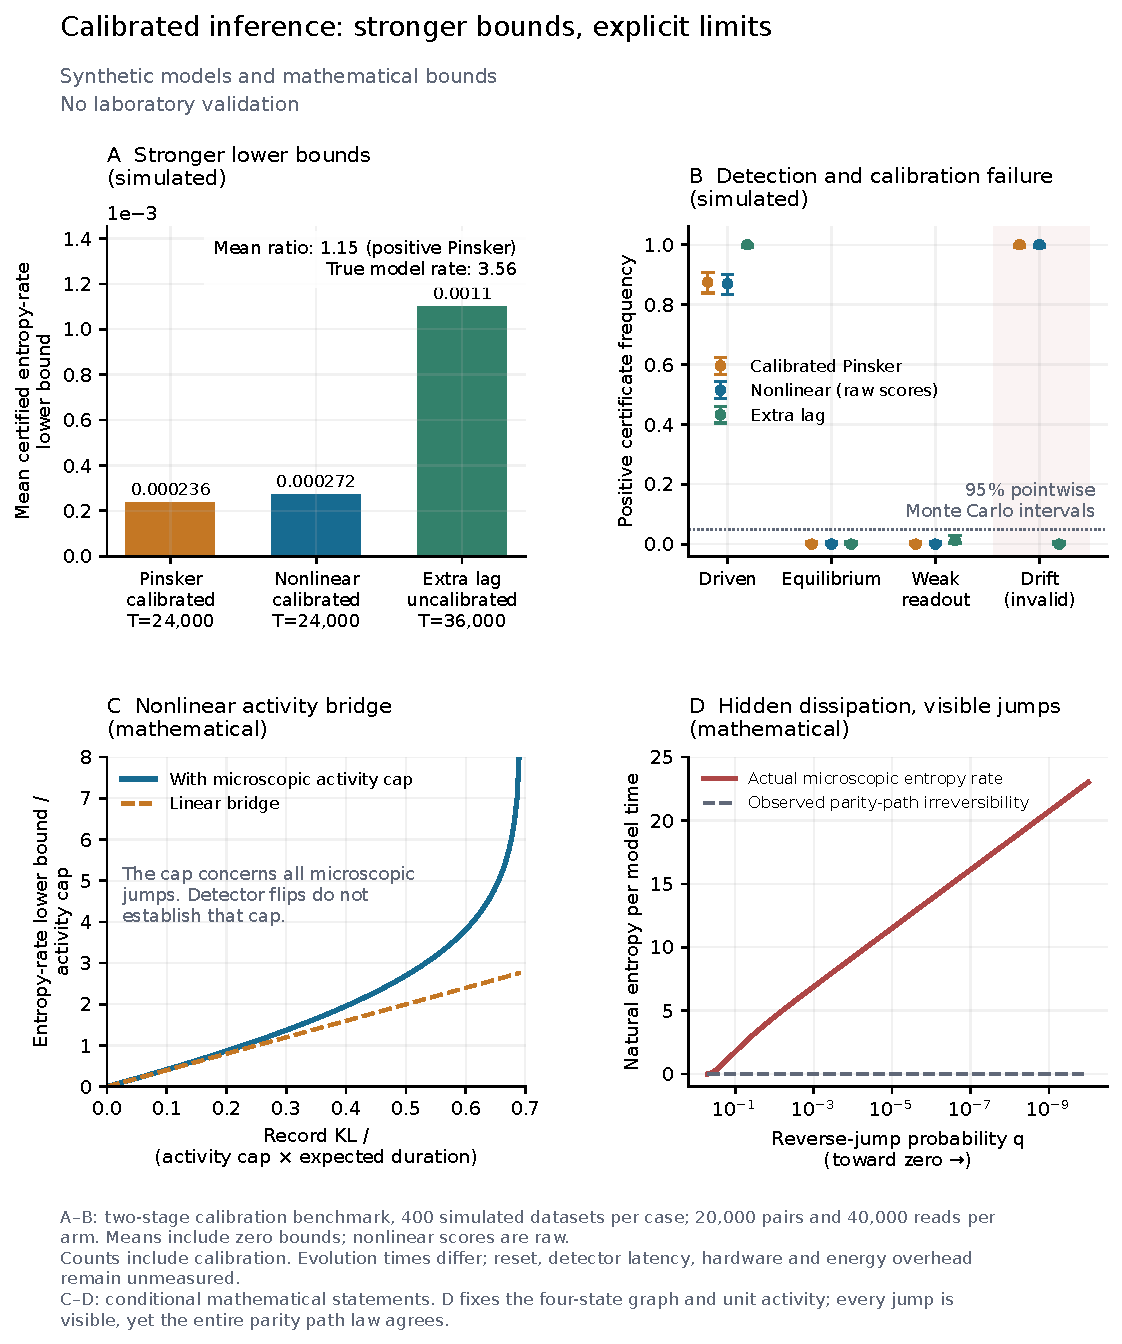
\includegraphics[width=\textwidth]{figures/calibrated_inference.pdf}
\caption{Calibrated inference and its limitations. The panels distinguish
an exact physical boundary, numerical information bounds and finite simulated
comparisons. The underlying records, equations and uncertainty calculations
are supplied in the following chapters and the release.}
\end{figure}
\begin{figure}[p]
\centering
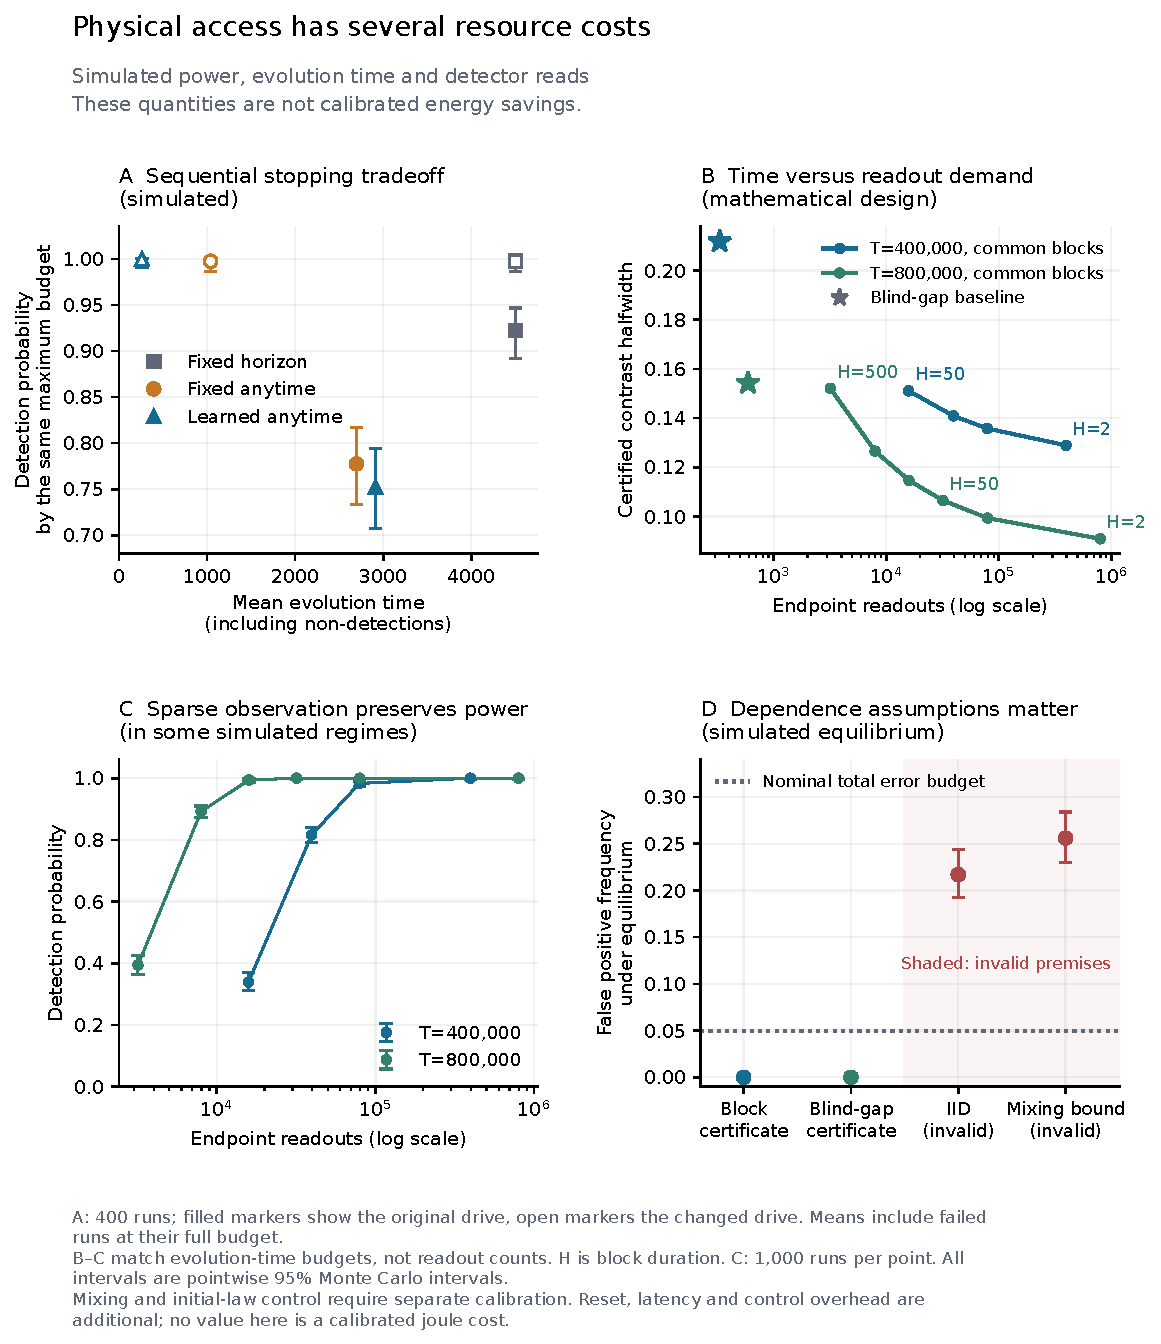
\includegraphics[width=\textwidth]{figures/calibrated_resources.pdf}
\caption{Acquisition choices at declared time and readout budgets. Each
simulated comparison is restricted to its frozen design. Faster stopping or
fewer readings does not imply a measured energy saving, and deliberately
invalid calibration controls remain part of the evaluation.}
\end{figure}
